The scope of this work includes development and demonstration of
various methods and tools to leverage Cyclus' existing
capabilities to model real-world fuel cycle transition scenarios.

\section{Background and motivation}
Increasing climate change concerns have directed attention
to nuclear energy, which produces reliable base load energy
with negligible CO$_2$ emission. With the reduction of fossil
fuel based power plants and the general increase in energy demand
(28\% growth between 2015 and 2040 \cite{conti_international_2016}),
nuclear power is expected to play a crucial role in the world energy portfolio.

However, concerns of the accumulating \gls{UNF} inventory,
safety of the current reactor fleet, and the availability of
uranium resources create a negative public perception of
nuclear energy and its sustainability.

\subsection{The Nuclear Fuel Cycle}
The nuclear fuel cycle is described as a set of facilities
that interact with one another to either provide or consume
fuel services \cite{gidden_agent-based_2015}. The goal of
the cycle is to produce power economically, while managing
the byproduct of power production, \gls{UNF}. The discharge
\gls{UNF} from the reactors are sent back to facilities for
either recycling or disposal. 

There are a large number of fuel cycle groups, categorized by the extent of recycling
(no recycle, limited recycle, and continuous recycle), elements and isotopes involved
(e.g. thorium-U233, uranium-plutonium), and the type of reactors (fast/thermal critical
reactors, sub-critical \gls{EDS}). The fuel cycle evaluation and screening study by
Wigeland et al. identified 40 evaluation groups \cite{wigeland_nuclear_2014}.

\subsubsection{Once-through fuel cycle}

The once-through cycle is when nuclear fuel is used once and then sent to 
storage without further reprocessing \cite{tsoulfanidis_nuclear_2013}.
This cycle is often called the open fuel cycle, and is the current cycle for
most nations with nuclear energy (e.g. U.S., Korea, Finland, Sweden).

The cycle begins with mining of uranium ore, which is extracted from the
ground. The mined ore is milled to form yellowcake ($U_3O_8$). From here,
the yellowcake is either converted to $UF_6$ and enriched, or converted
to $UO_2$ directly. This is because some reactor designs (e.g. \glspl{CANDU} \cite{torgerson_candu_2006})
can operate with natural uranium, while others (e.g. \glspl{PWR}) needs
higher-than-natural levels of uranium-235. The processed $UO_2$ is
then fabricated to pellets and loaded into fuel assemblies. 

Once the fuel is depleted in the reactor, it is put in pools to cool down.
This process ranges from two to seven years. After cooling, the \gls{UNF}
is stored in dry casks as interim storage, destined to be sent to a geologic repository
for permanent disposal.

\subsubsection{Closed Fuel Cycle}
A closed fuel cycle is when the \gls{UNF} is recycled to be reused
in a nuclear reactor. Recycling is not adopted worldwide due to
its concerns of high cost and proliferation, but has two major
benefits: increase fuel utilization and reduction of repository
burden. 

\gls{UNF} discharged from a typical \gls{LWR} has an approximate
composition as the following: 95\% uranium, 1\% plutonium, 0.1\%
minor actinides, 4\% fission products \cite{feiveson_spent_2011}.
The uranium, plutonium, and the minor actinides have the capability
to produce power through fission. Thus, every group except the
minor actinides can be separated to create new fuel for other reactors.

Additionally, repository capacity is constrained mostly by decay heat
load and radioactivity, meaning that removal of the high-activity
isotopes can accomplish a more efficient utilization of the repository
capacity. Short-lived fission products (e.g. cesium, strontium) contribute
to a large heat and radioactivity in the first 100 years of \gls{UNF} disposal,
and minor actinides (americium, plutonium), with their long half-lives,
contribute to longer-term heat and radioactivity in the repository \cite{wigeland_separations_2006},
as shown in figure \ref{fig:decay_heat}.


\begin{figure}[htbp!]
	\begin{center}
		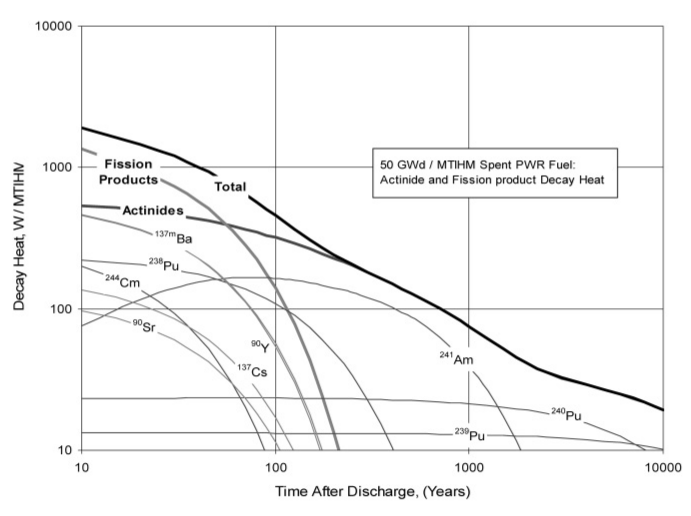
\includegraphics[scale=0.3]{./images/decay_heat.png}
	\end{center}
	\caption{Decay heat contributions in \gls{UNF} from a \gls{PWR} irradiated
		to 50 GWd/MTHM \cite{wigeland_separations_2006}.}
	\label{fig:decay_heat}
\end{figure}


There are two major reprocessing technologies:
methods that use low-temperature chemical separation
using organic solvents (e.g. PUREX \cite{baumgaertner_purex_1976}), and
methods that use high-temperature molten salts and metals, like pyroprocessing
\cite{laidler_development_1997}. These methods separate the \gls{UNF}
into different streams, which are then sent to either a \gls{HLW} repository
(fission products) or an appropriate fuel fabrication facility (plutonium).

Different closed fuel cycles use different elemental groups for recycled
fuel fabrication. For example, the PUREX process is used in La Hague in France
\cite{schneider_spent_2008}, THORP in the U.K \cite{riley_technology_1998},
Mayak in Russia, and Rokkasho in Japan to separated plutonium and uranium
\cite{birkett_recent_2005}. The plutonium is mixed with either depleted
uranium (tails) or reprocessed uranium to produced \gls{MOX}. France
uses \gls{MOX} fuel for its \glspl{LWR}, but closed fuel cycles 
generally involve fast-spectrum reactors to control TRU inventory.
A fast-spectrum reactor can be designed to either burn (reduce TRU),
breed (produce more TRU), or break-even (maintain TRU amount).

The closed fuel cycle types deployed in this work uses breeder reactors,
with a U-Pu fuel cycle. The goal of breeder
reactors is to eliminate the need for natural uranium, and
increase resource utilization by recycling depleted uranium and \gls{UNF}.


\section{Objectives}

This thesis demonstrates real-world \gls{NFC} transition
scenario modeling capabilities of Cyclus. The first objective is
to benchmark Cyclus to other fuel cycle simulation tools to
show that Cyclus' results are in good agreement with the results
from other codes. The second objective is to develop tools
necessary to model real-world \gls{NFC} transition
scenarios. The tools include a script that creates a Cyclus
input file of the historical nuclear reactor operation from
a database, and a module that models \gls{MSR} behavior in Cyclus.
Finally, I use Cyclus to construct a simulation of the nuclear
fuel cycle transition scenario for France and the United States,
to obtain metrics such as \gls{UNF} and raffinate inventory.


\section{Methods}
This thesis accomplishes the objective in three steps. First,
the general fuel cycle simulation tool, Cyclus, is benchmarked
to demonstrate its agreement with other fuel cycle simulation
tools. Second, I identify the tools and methods necessary
for modeling and simulating real-world transition scenarios.
Finally, I construct and run fuel cycle transition scenarios
for France and the United States.

A previous study \cite{feng_standardized_2016} validates existing fuel cycle
simulation tools in a fuel cycle transition scenario, where a \gls{LWR} fleet
transitions into an \gls{SFR} fleet with continuous reprocessing. This 
study compares four well-known \glspl{NFCS}
DYMOND \cite{yacout_modeling_2005},
VISION \cite{jacobson_verifiable_2010},
ORION \cite{gregg_analysis_2012}, and
MARKAL \cite{shay_epa_2006}. The results from each code were
compared to a set of `model solutions' that were generated
from an excel worksheet for different metrics (e.g. fuel loading
in reactor, \gls{UNF} inventory). I reproduce the transition
scenario on Cyclus, and compare the Cyclus results with those
from the `model solutions'.

In order to model real-world transition scenarios into an advanced
fuel cycle, I developed two major tools. First, I developed a python
module that automates extraction from the curated \gls{IAEA} \gls{PRIS} database
\cite{iaea_nuclear_2018}. The database lists each nuclear reactor's
country, name, type, net capacity (\gls{MWe}), status, operator, construction
date, first criticality date, first grid date, commercial date, and shutdown
date (if applicable). The module extracts the information from this file
to generate a Cyclus compatible input file, which lists the individual
reactor units as agents. Second, I developed a tool that models \glspl{MSR}
using a database generated from a high-fidelity \gls{MSR} depletion calculation.
The database is an output of Saltproc [!!! Cite saltproc], a python
module that drives
SERPENT 2 \cite{leppanen_serpentcontinuous-energy_2013} to model on-line reprocessing in an \gls{MSR}.
The hdf5 database contains isotopic timeseries of streams in and out of the reactor,
isotopic timeseries inside the reactor, and keff values. The developed tool then
reads the hdf5 file to mimic \gls{MSR} behavior by requesting and offering
material to the Cyclus framework.

Finally I construct the fuel cycle transition scenario for France and the United States.
I make different assumptions for the two scenarios due to each nation's different goals,
initial conditions (currently existing fleet, \gls{UNF} inventory), and their pursued reactor
technology.

The structure of this thesis is as follows. In chapter 2, I review other fuel cycle simulation
tools and their gaps, and explain why Cyclus
has the unique capability for modeling real-world fuel cycle transition scenarios.
Chapter 3 contains explanation and development of the tools that add the 
capabilities needed to accomplish the objective.
In chapter 4, I list and justify my assumption for the fuel cycle transition
scenario for France and the United States.
Chapter 5 shows the results from the benchmark study, where Cyclus results are compared
to results from other fuel cycle simulation tools.
Chapter 6 and 7 shows the results from the France and United States fuel cycle transition
scenario.

\iffalse
For France, I model the entire \gls{EU} region to calculate \gls{UNF} inventory
in each \gls{EU} nation. This is because France would need to receive \gls{UNF} from other
nations to quickly transition into a \gls{SFR} fleet, since their \gls{UNF} inventory
is small due to their long history of reprocessing for \gls{LWR} \gls{MOX} fuel production.
\fi

